\chapter{Results}

In this chapter, the results of the previously described algorithms will be discussed. Generally, all black lines are drawn with the rake down, and the red lines are the connection paths where the BeachBot is driving with the rake in upper position. The post processing is \textit{not} applied in these images.

\section{Verifying LKH Solutions}

To verify that the TSP solver produces viable output and that the tour postprocessing works, two simple test images are presented in \autoref{fig:ver_tsp}.

\begin{figure}
\begin{subfigure}[b]{0.45\textwidth}
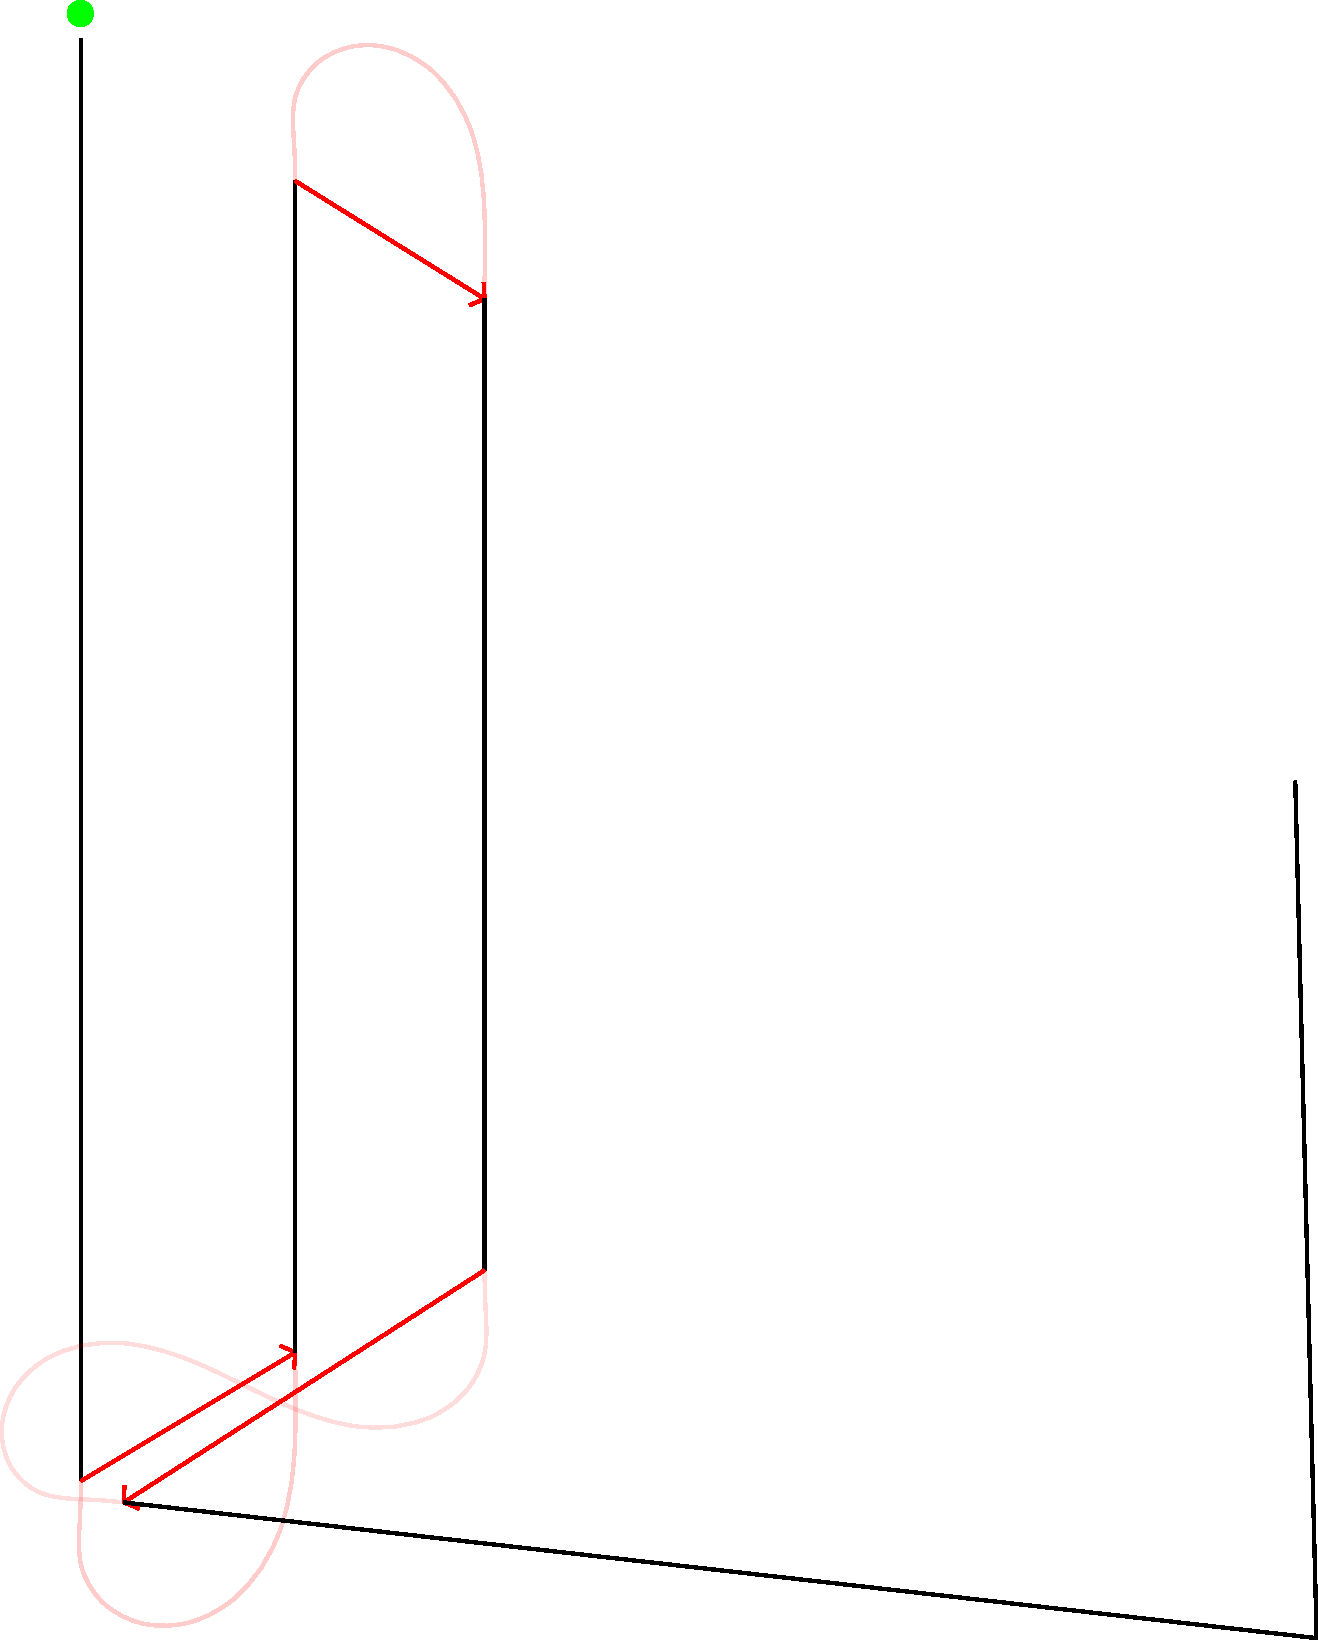
\includegraphics[width=1\textwidth]{images/results/TSP/TSP_Verification_1.pdf}
\caption{The red arrows show the tour: The nearest neighbour is not chosen and a more global optimum is obtained.}
\end{subfigure}
~
\begin{subfigure}[b]{0.45\textwidth}
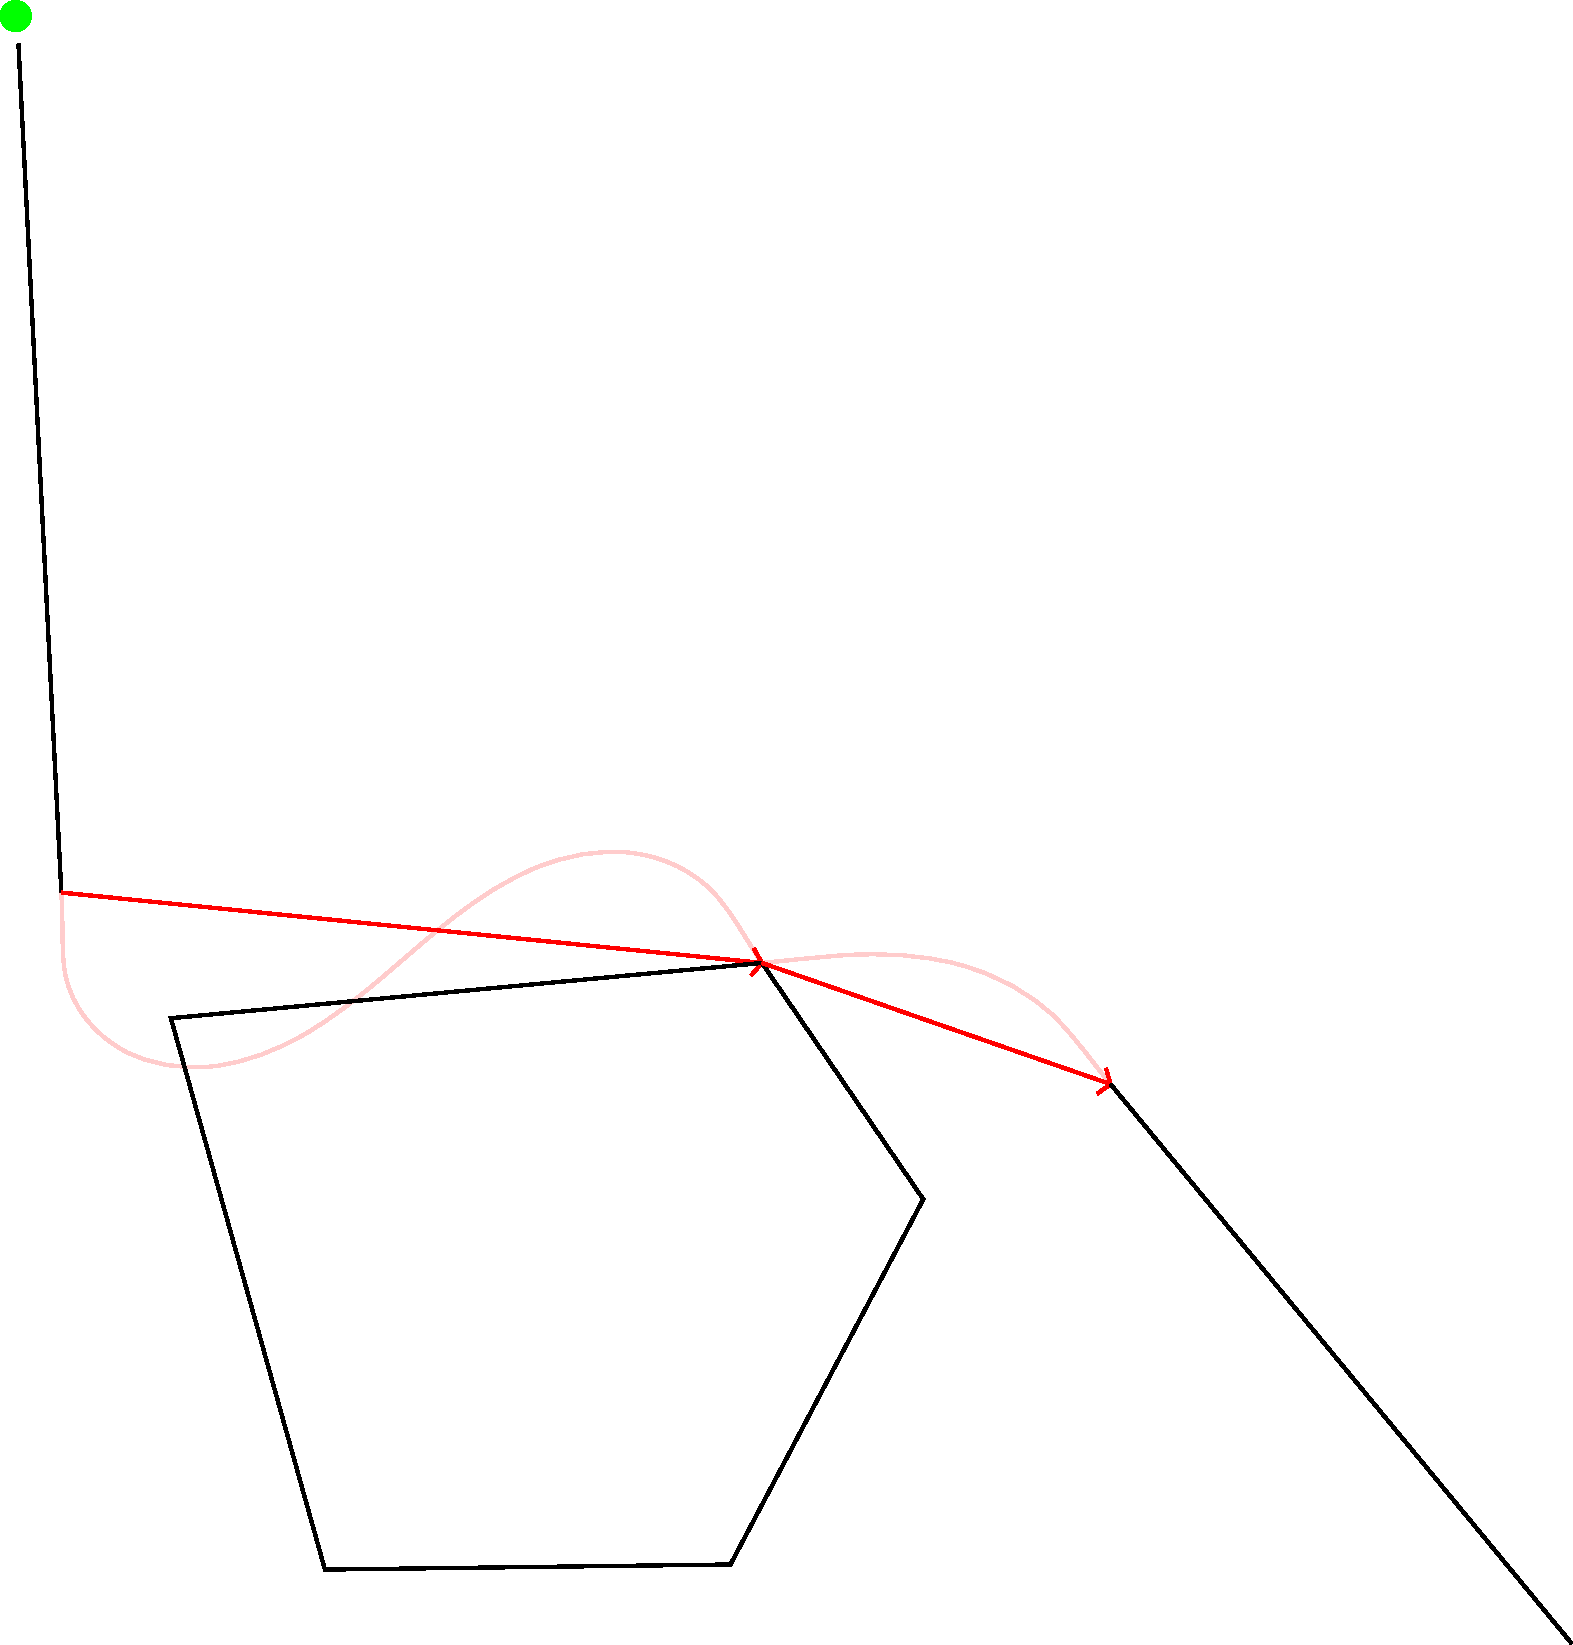
\includegraphics[width=1\textwidth]{images/results/TSP/TSP_Verification_2.pdf}
\caption{Again, not the nearest vertex on the polygon is chosen but rather a vertex where the global tour distance is minimized.}
\end{subfigure}
\caption{Verifying that the Traveling Salesman solver produces viable solutions.}\label{fig:ver_tsp}
\end{figure}

\clearpage
\section{Line Drawings}

Line drawings consist of no filled areas. This type of drawing is easily created manually and therefore we have used them extensively during testing. The solutions of the manual drawings (with manual connections) are compared to the solutions generated by the algorithm.

\subsection{The Lion Drawing}

The lion was one of the earliest drawings that the BeachBot was able to reproduce on the beach canvas. It is also available as part of the distributed source of the application (\texttt{assets/lion\_example.svg}).

\begin{figure}[h]
\begin{subfigure}[t]{0.45\textwidth}
	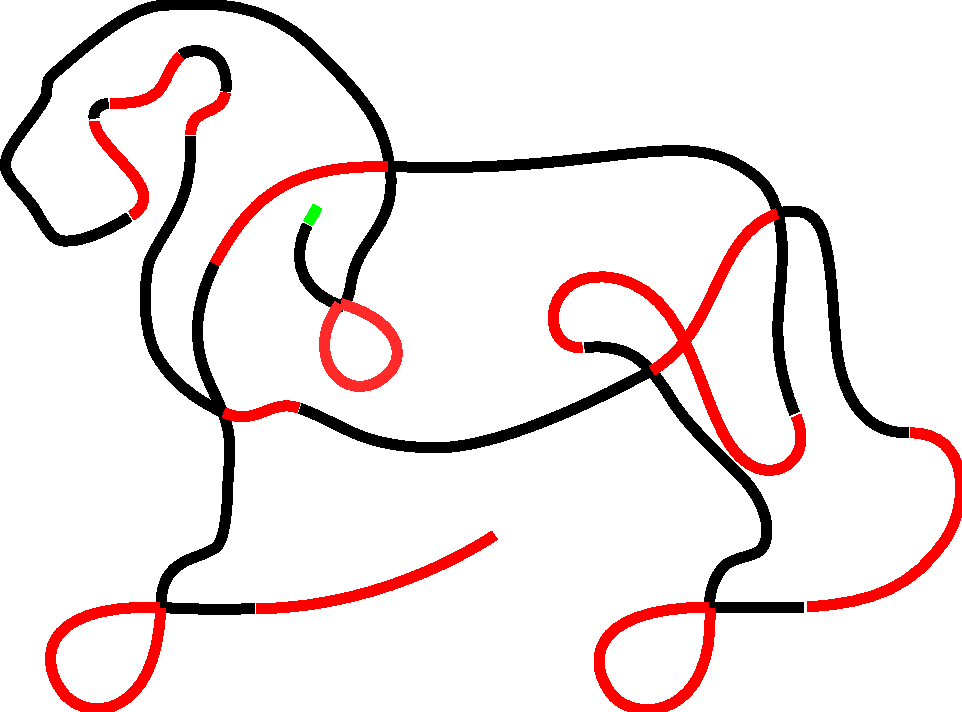
\includegraphics[width=\textwidth]{images/results/lion/lion_handmade.pdf}
	\caption{Reference lion drawing created manually}
\end{subfigure}
\begin{subfigure}[t]{0.45\textwidth}
	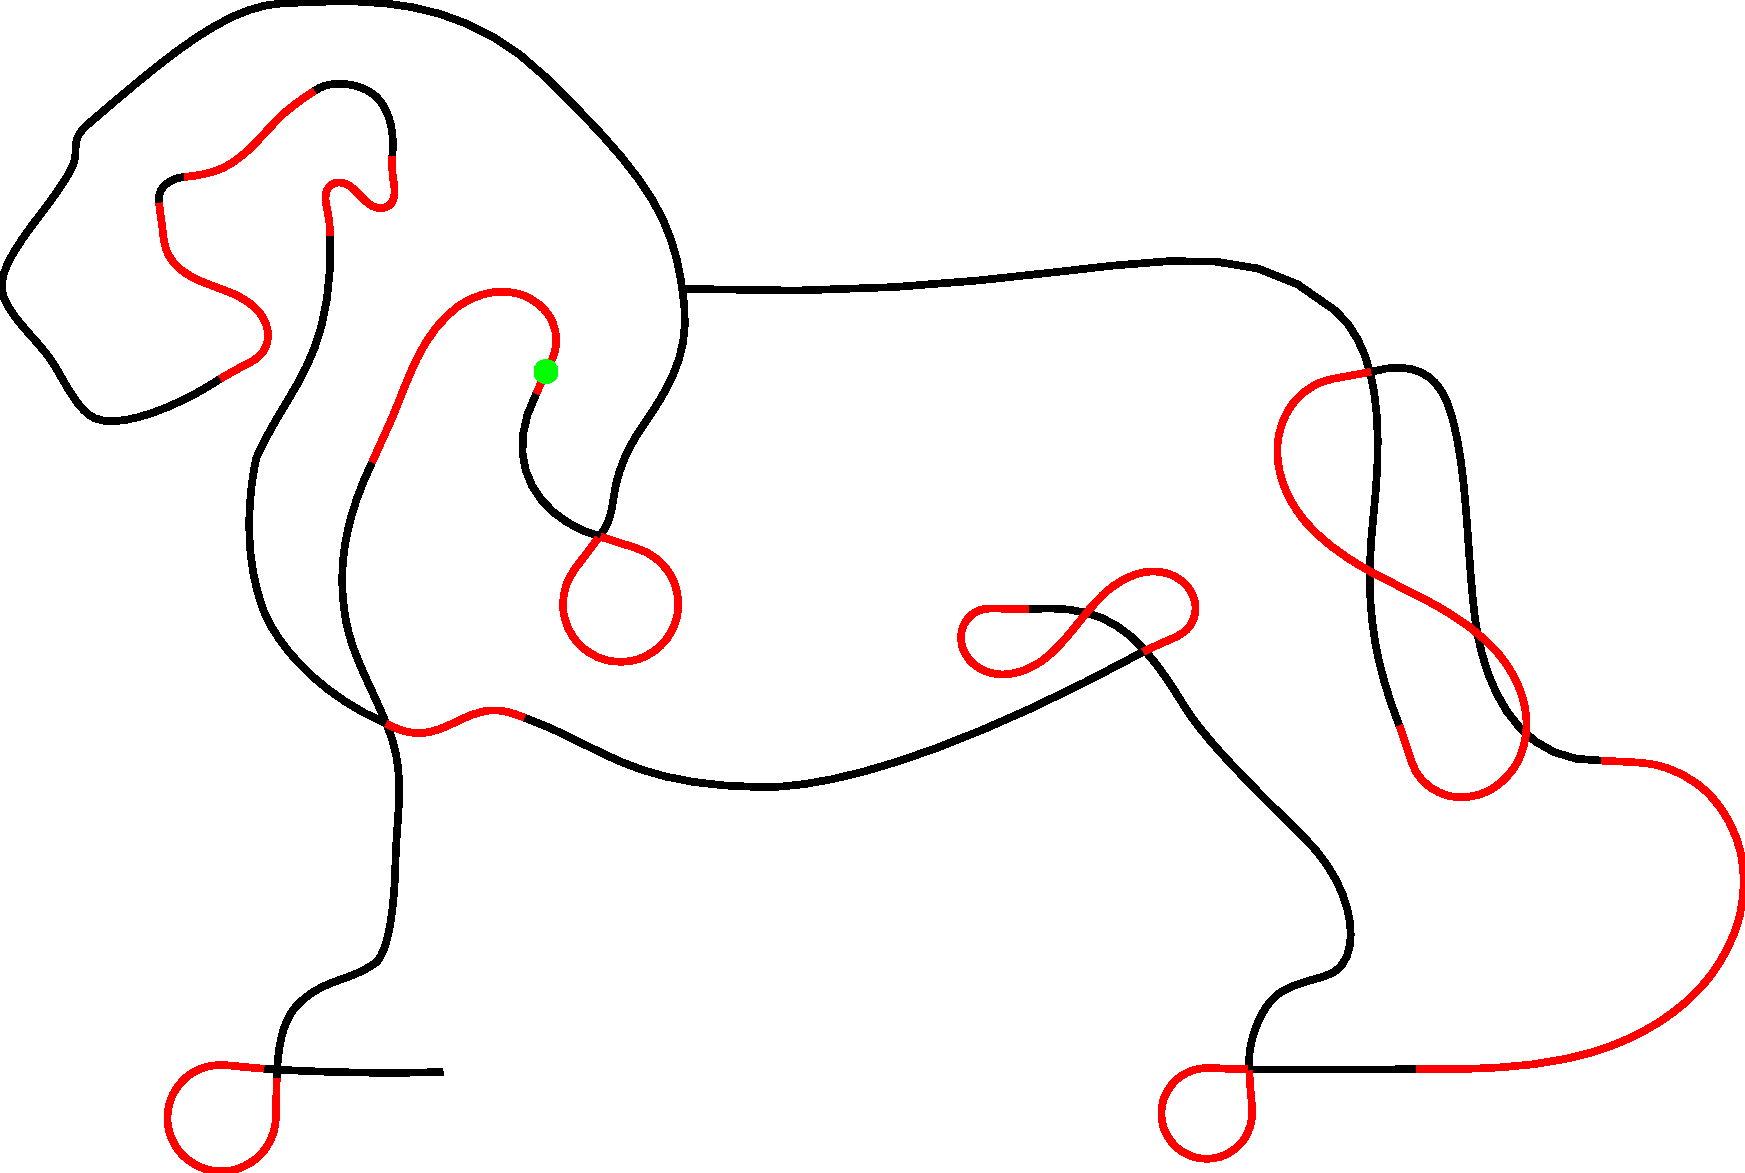
\includegraphics[width=\textwidth]{images/results/lion/lion_generated_22.pdf}
	\caption{Generated by the generator algorithm}
\end{subfigure}
\par\bigskip % force a bit of vertical whitespace
\begin{subfigure}[t]{0.45\textwidth}
	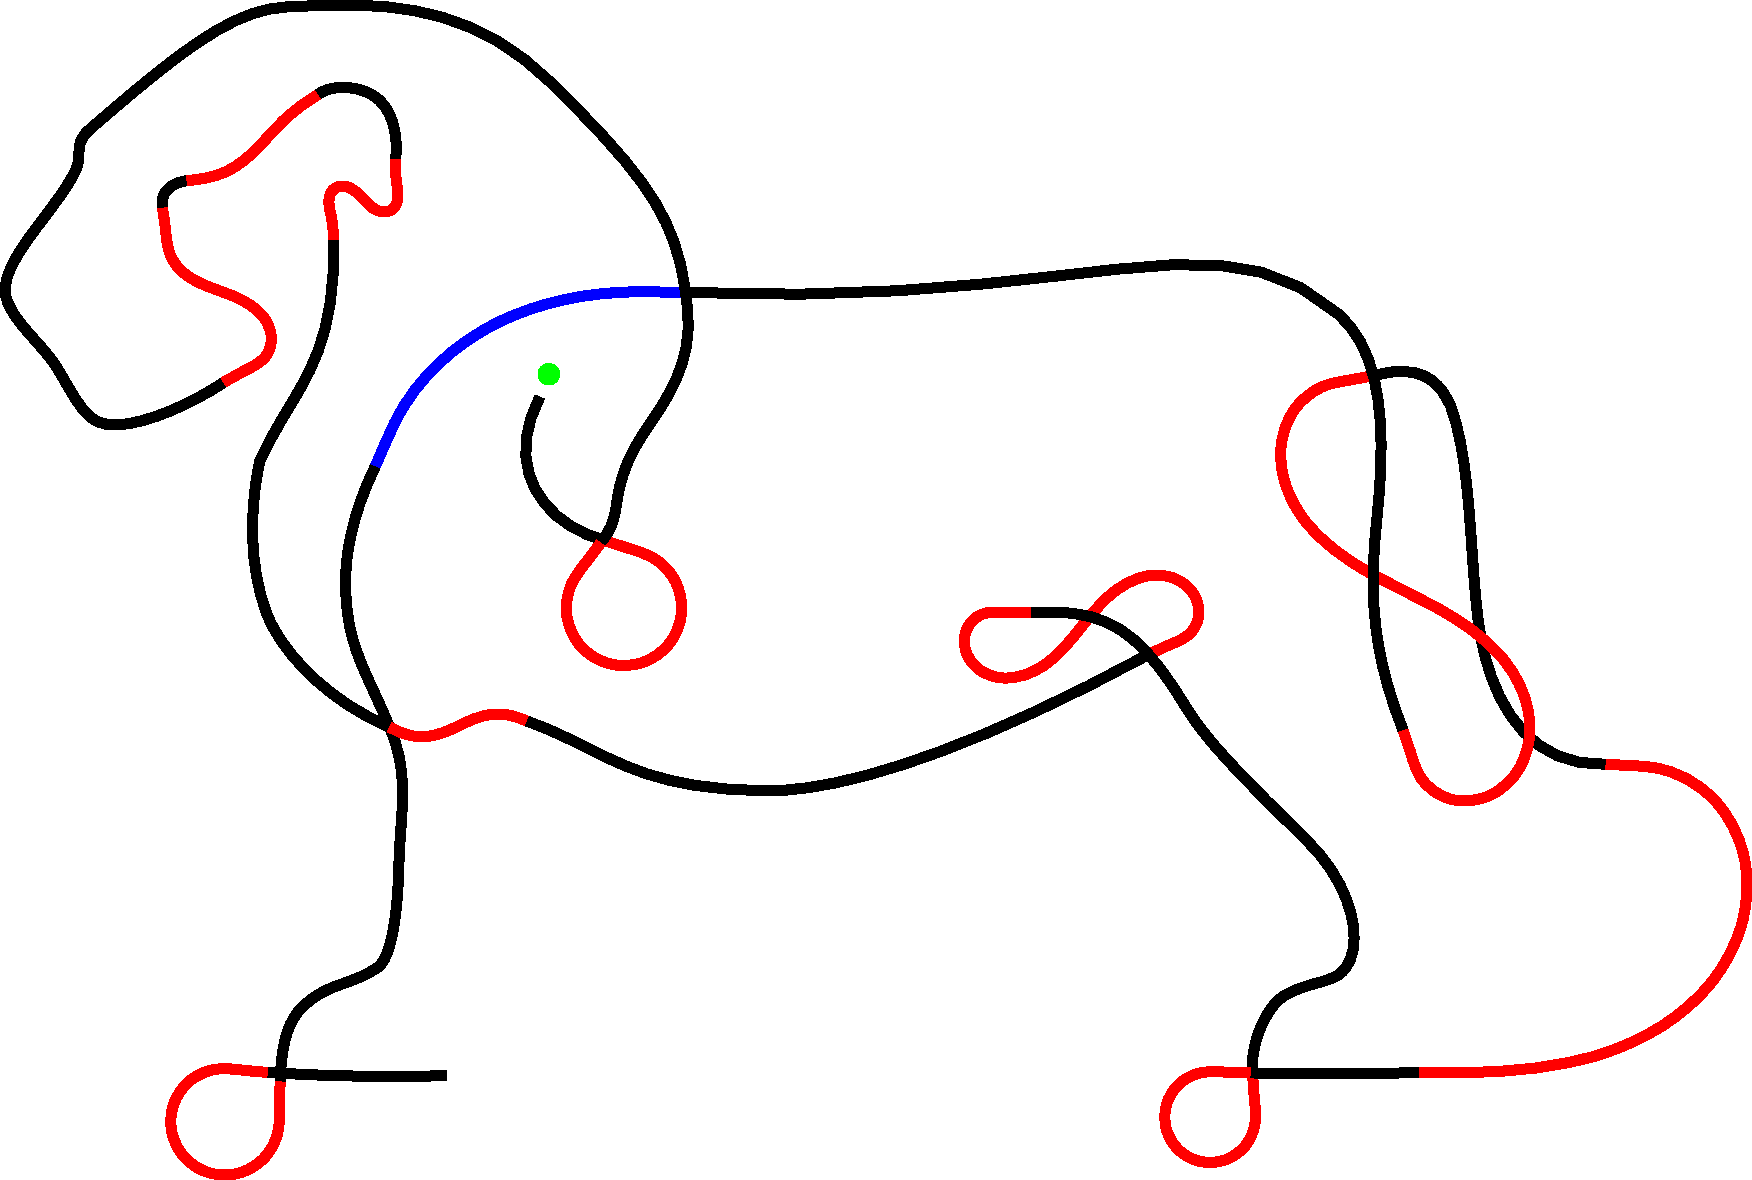
\includegraphics[width=\textwidth]{images/results/lion/lion_generated_enforced_connection.pdf}
	\caption{Generated, with enforcement of one connection (blue).}
\end{subfigure}
\begin{subfigure}[t]{0.45\textwidth}
	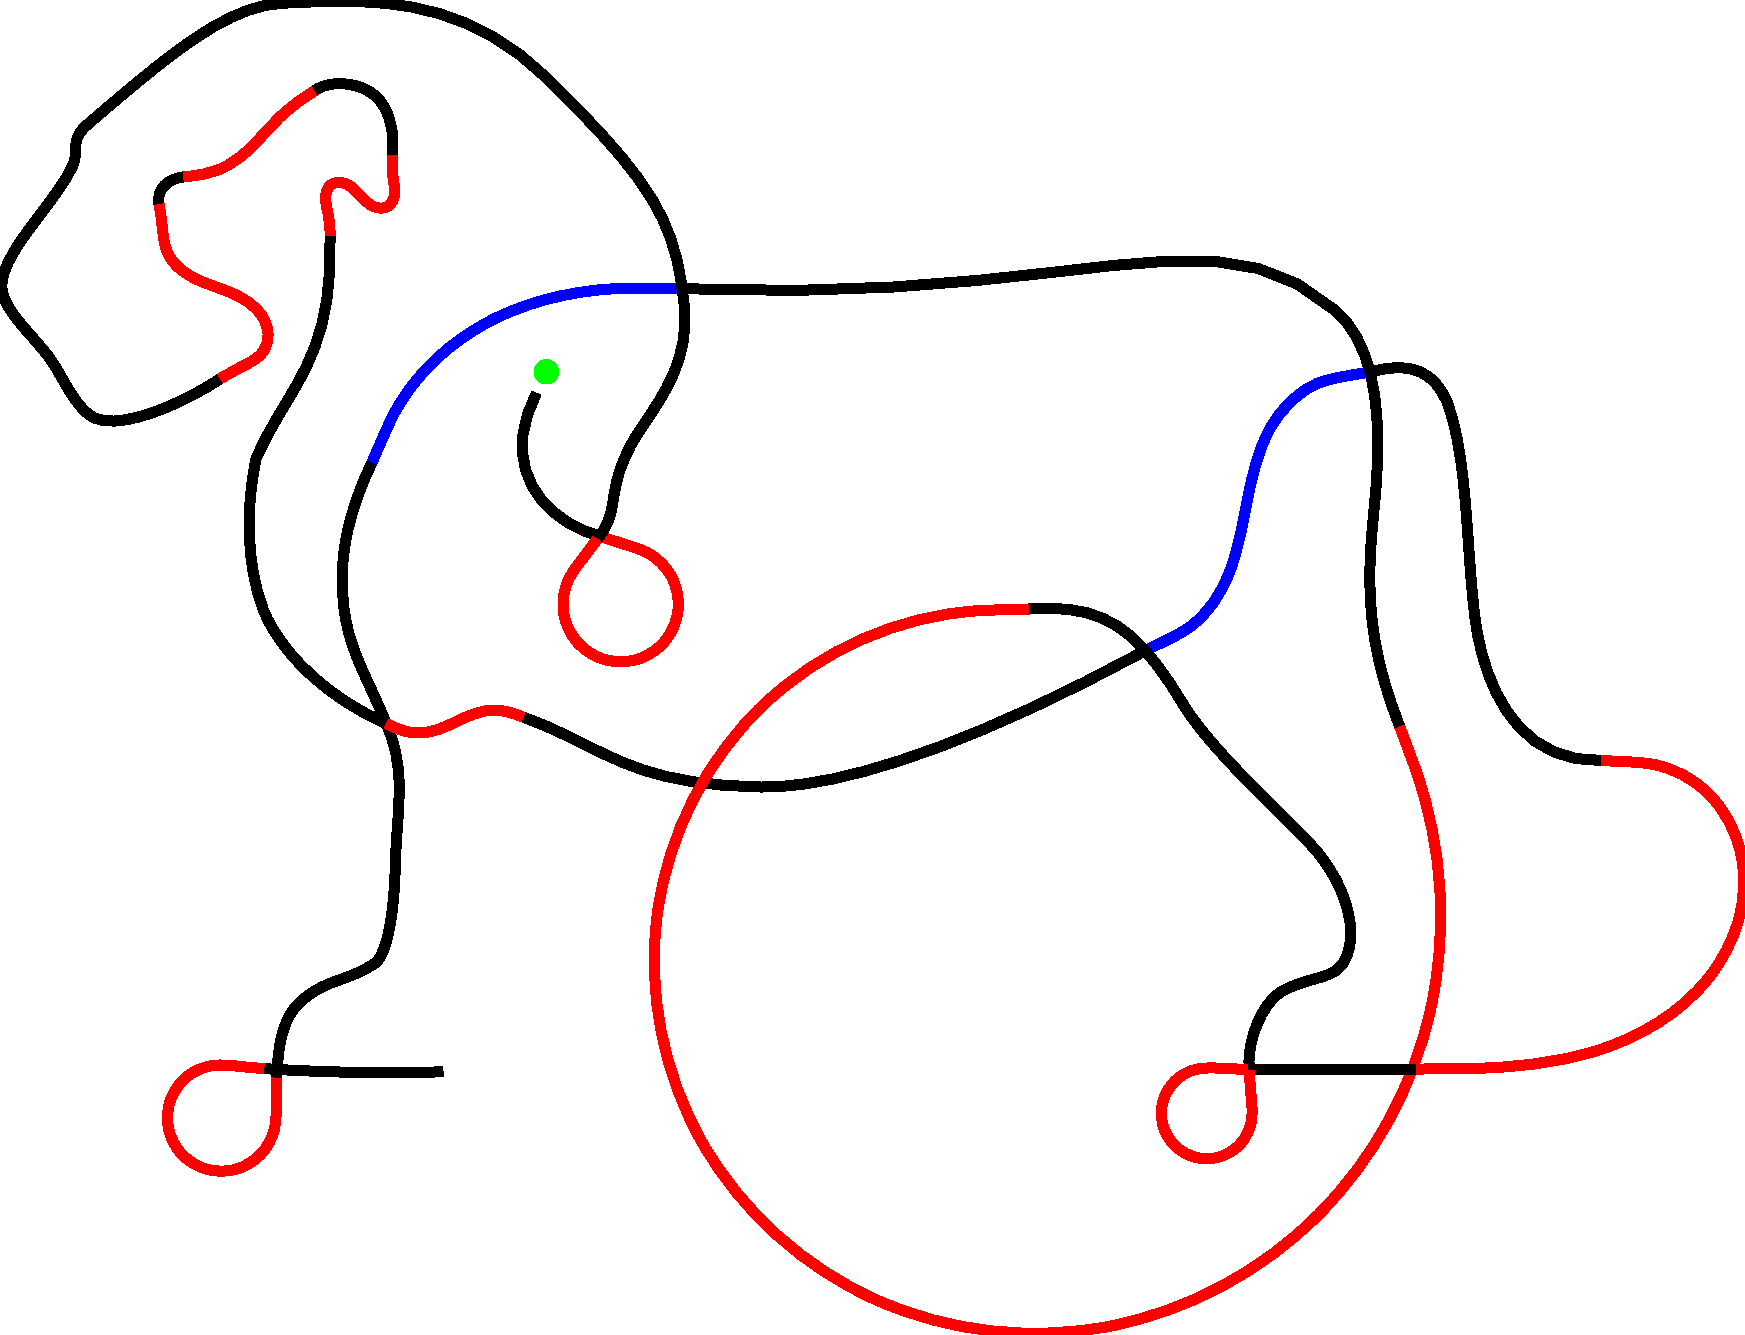
\includegraphics[width=\textwidth]{images/results/lion/lion_generated_enforced_connection_with_degen.pdf}
	\caption{Generated, with two enforced connections. With the unimproved spiro control point heuristic, there is one larger circular connection visible.}
\end{subfigure}\\
\centering
\begin{subfigure}[t]{0.8\textwidth}
	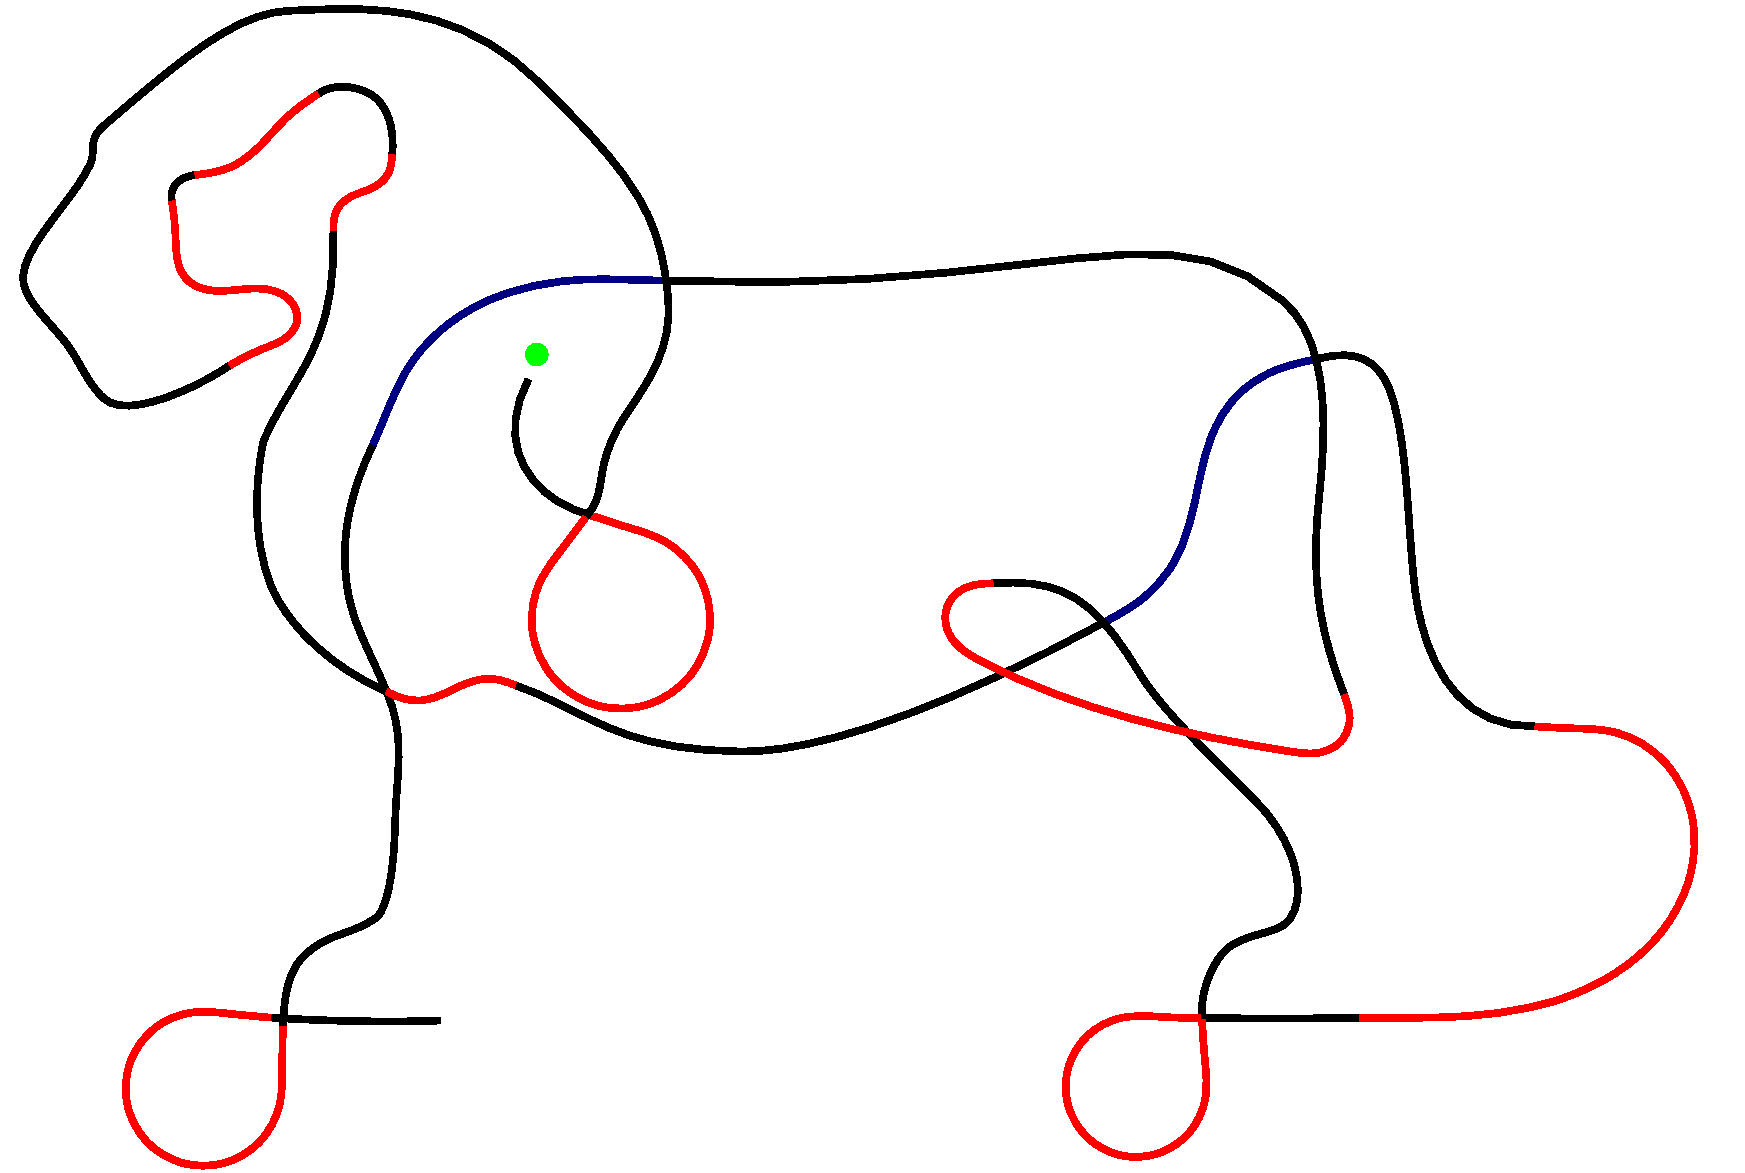
\includegraphics[width=\textwidth]{images/results/lion/lion_new_heuristic2.pdf}
	\caption{With the improved spiro control point heuristic, the huge circular connection is not present anymore (\enquote{curvature} limit is also slightly higher). The connection between neck and ear is also smoother, now.}
\end{subfigure}

\caption{Comparison of manual and automatically generated lion trajectory}
\end{figure}

\clearpage

\subsection{The Shark Drawing}

Another line drawing, with a closed polygon, is the \enquote{Danger, Sharks} drawing.

\begin{figure}[h]
\centering
\begin{subfigure}[t]{0.45\textwidth}
	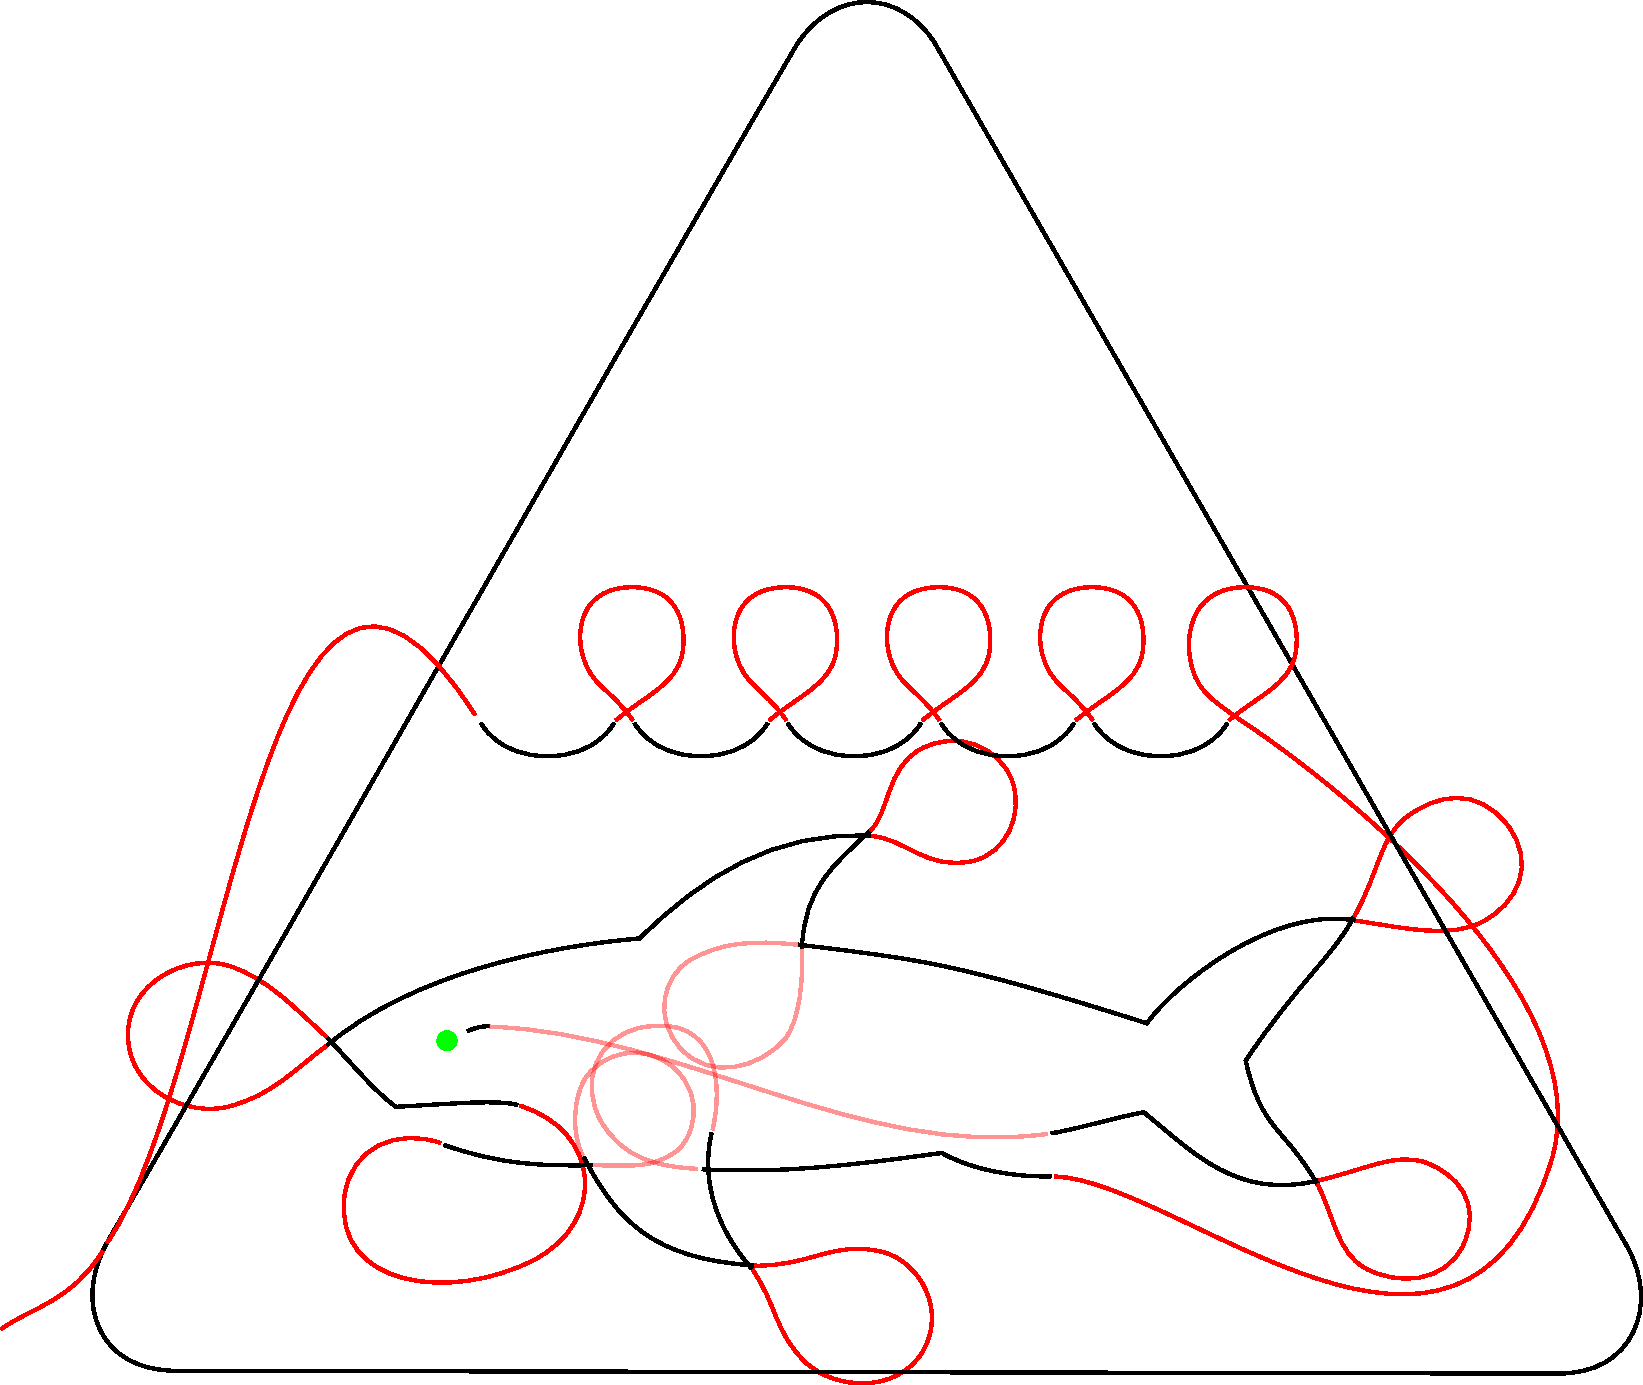
\includegraphics[width=\textwidth]{images/results/shark/hai_achtung.pdf}
	\caption{The manually created reference image.}
\end{subfigure}~
\begin{subfigure}[t]{0.45\textwidth}
	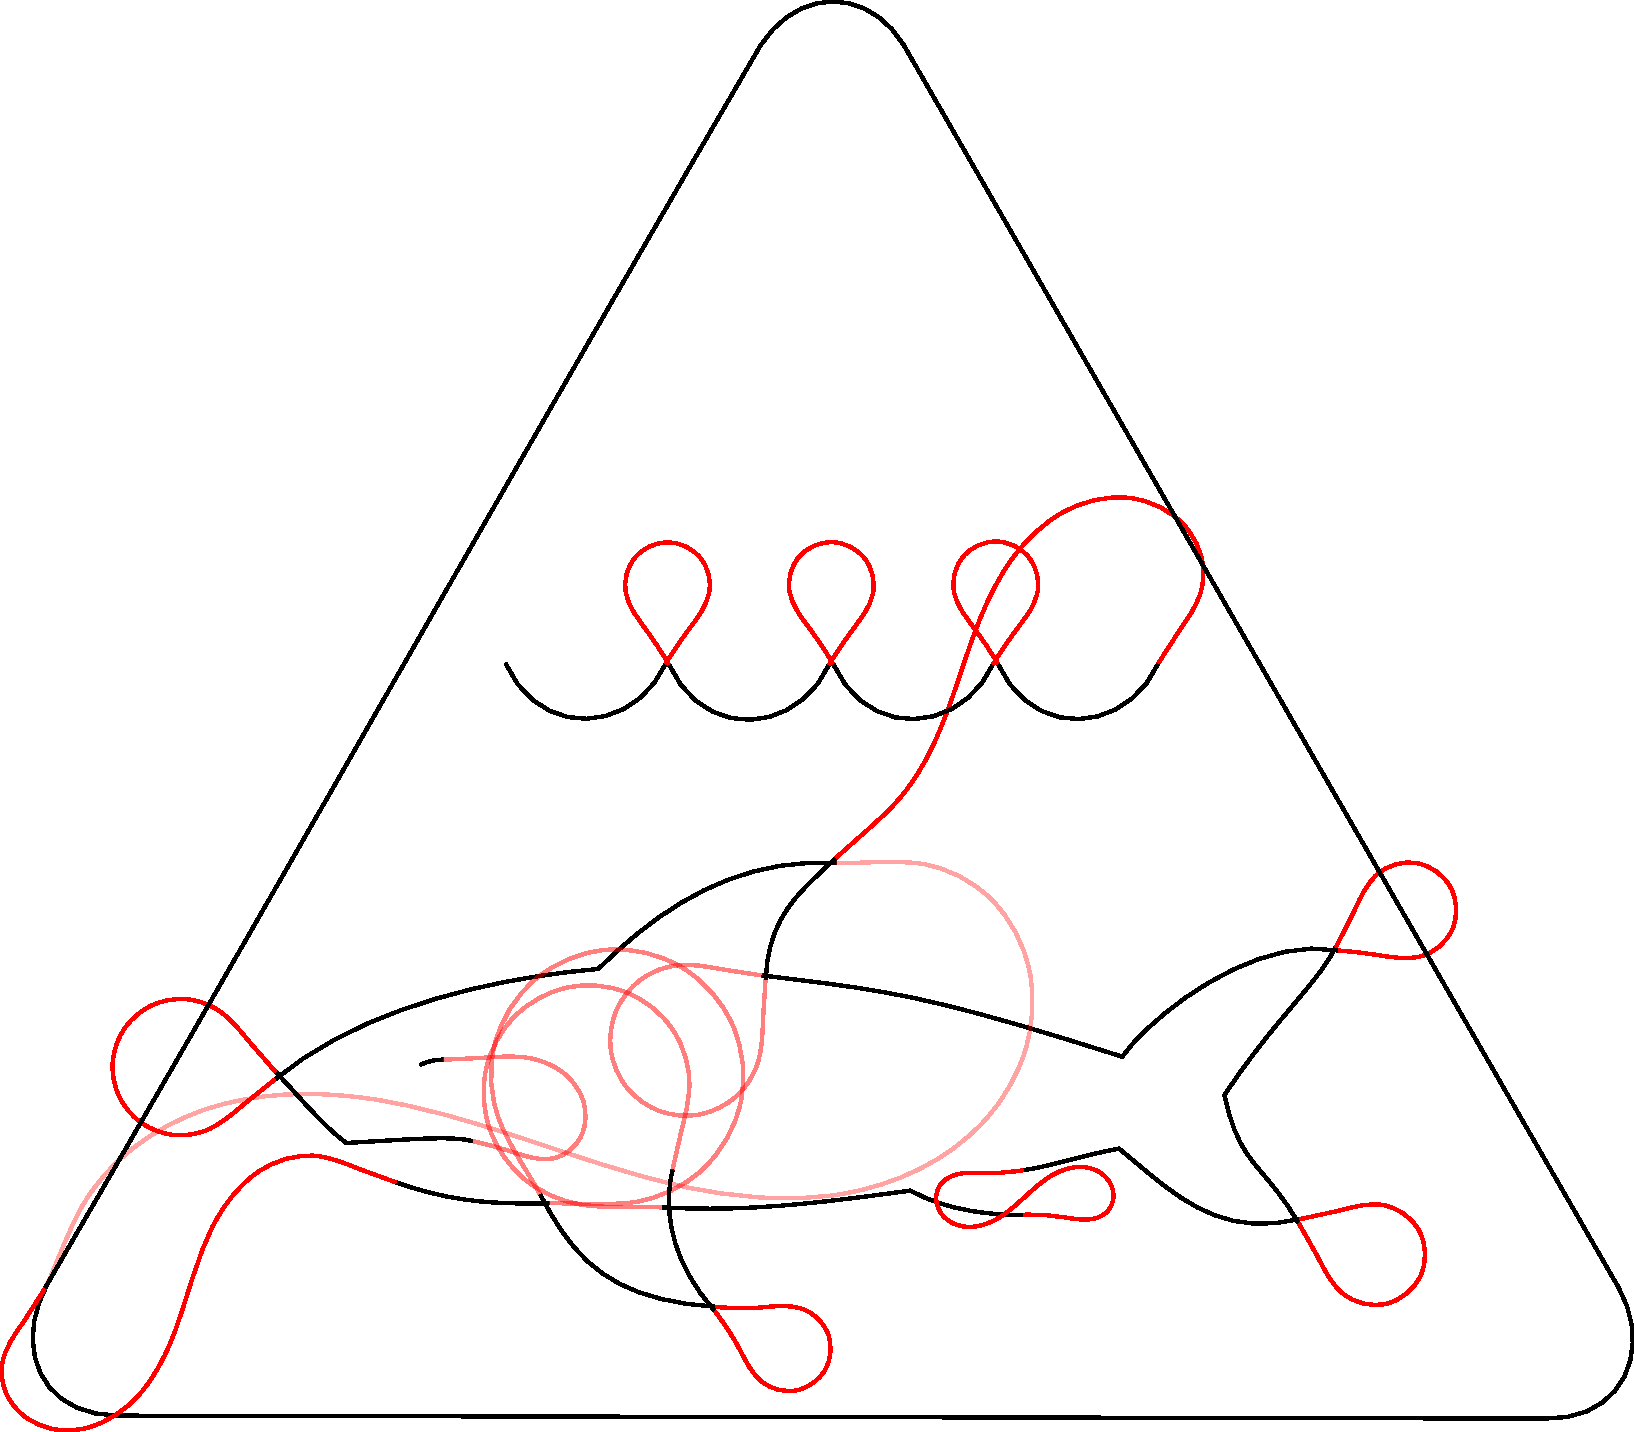
\includegraphics[width=\textwidth]{images/results/shark/export_hai_new.pdf}
	\caption{Generated by the path generator: Note how the \enquote{outer} polygon is visited previous to finishing the inner drawing.}
\end{subfigure}
\par\bigskip
\begin{subfigure}[t]{0.8\textwidth}
	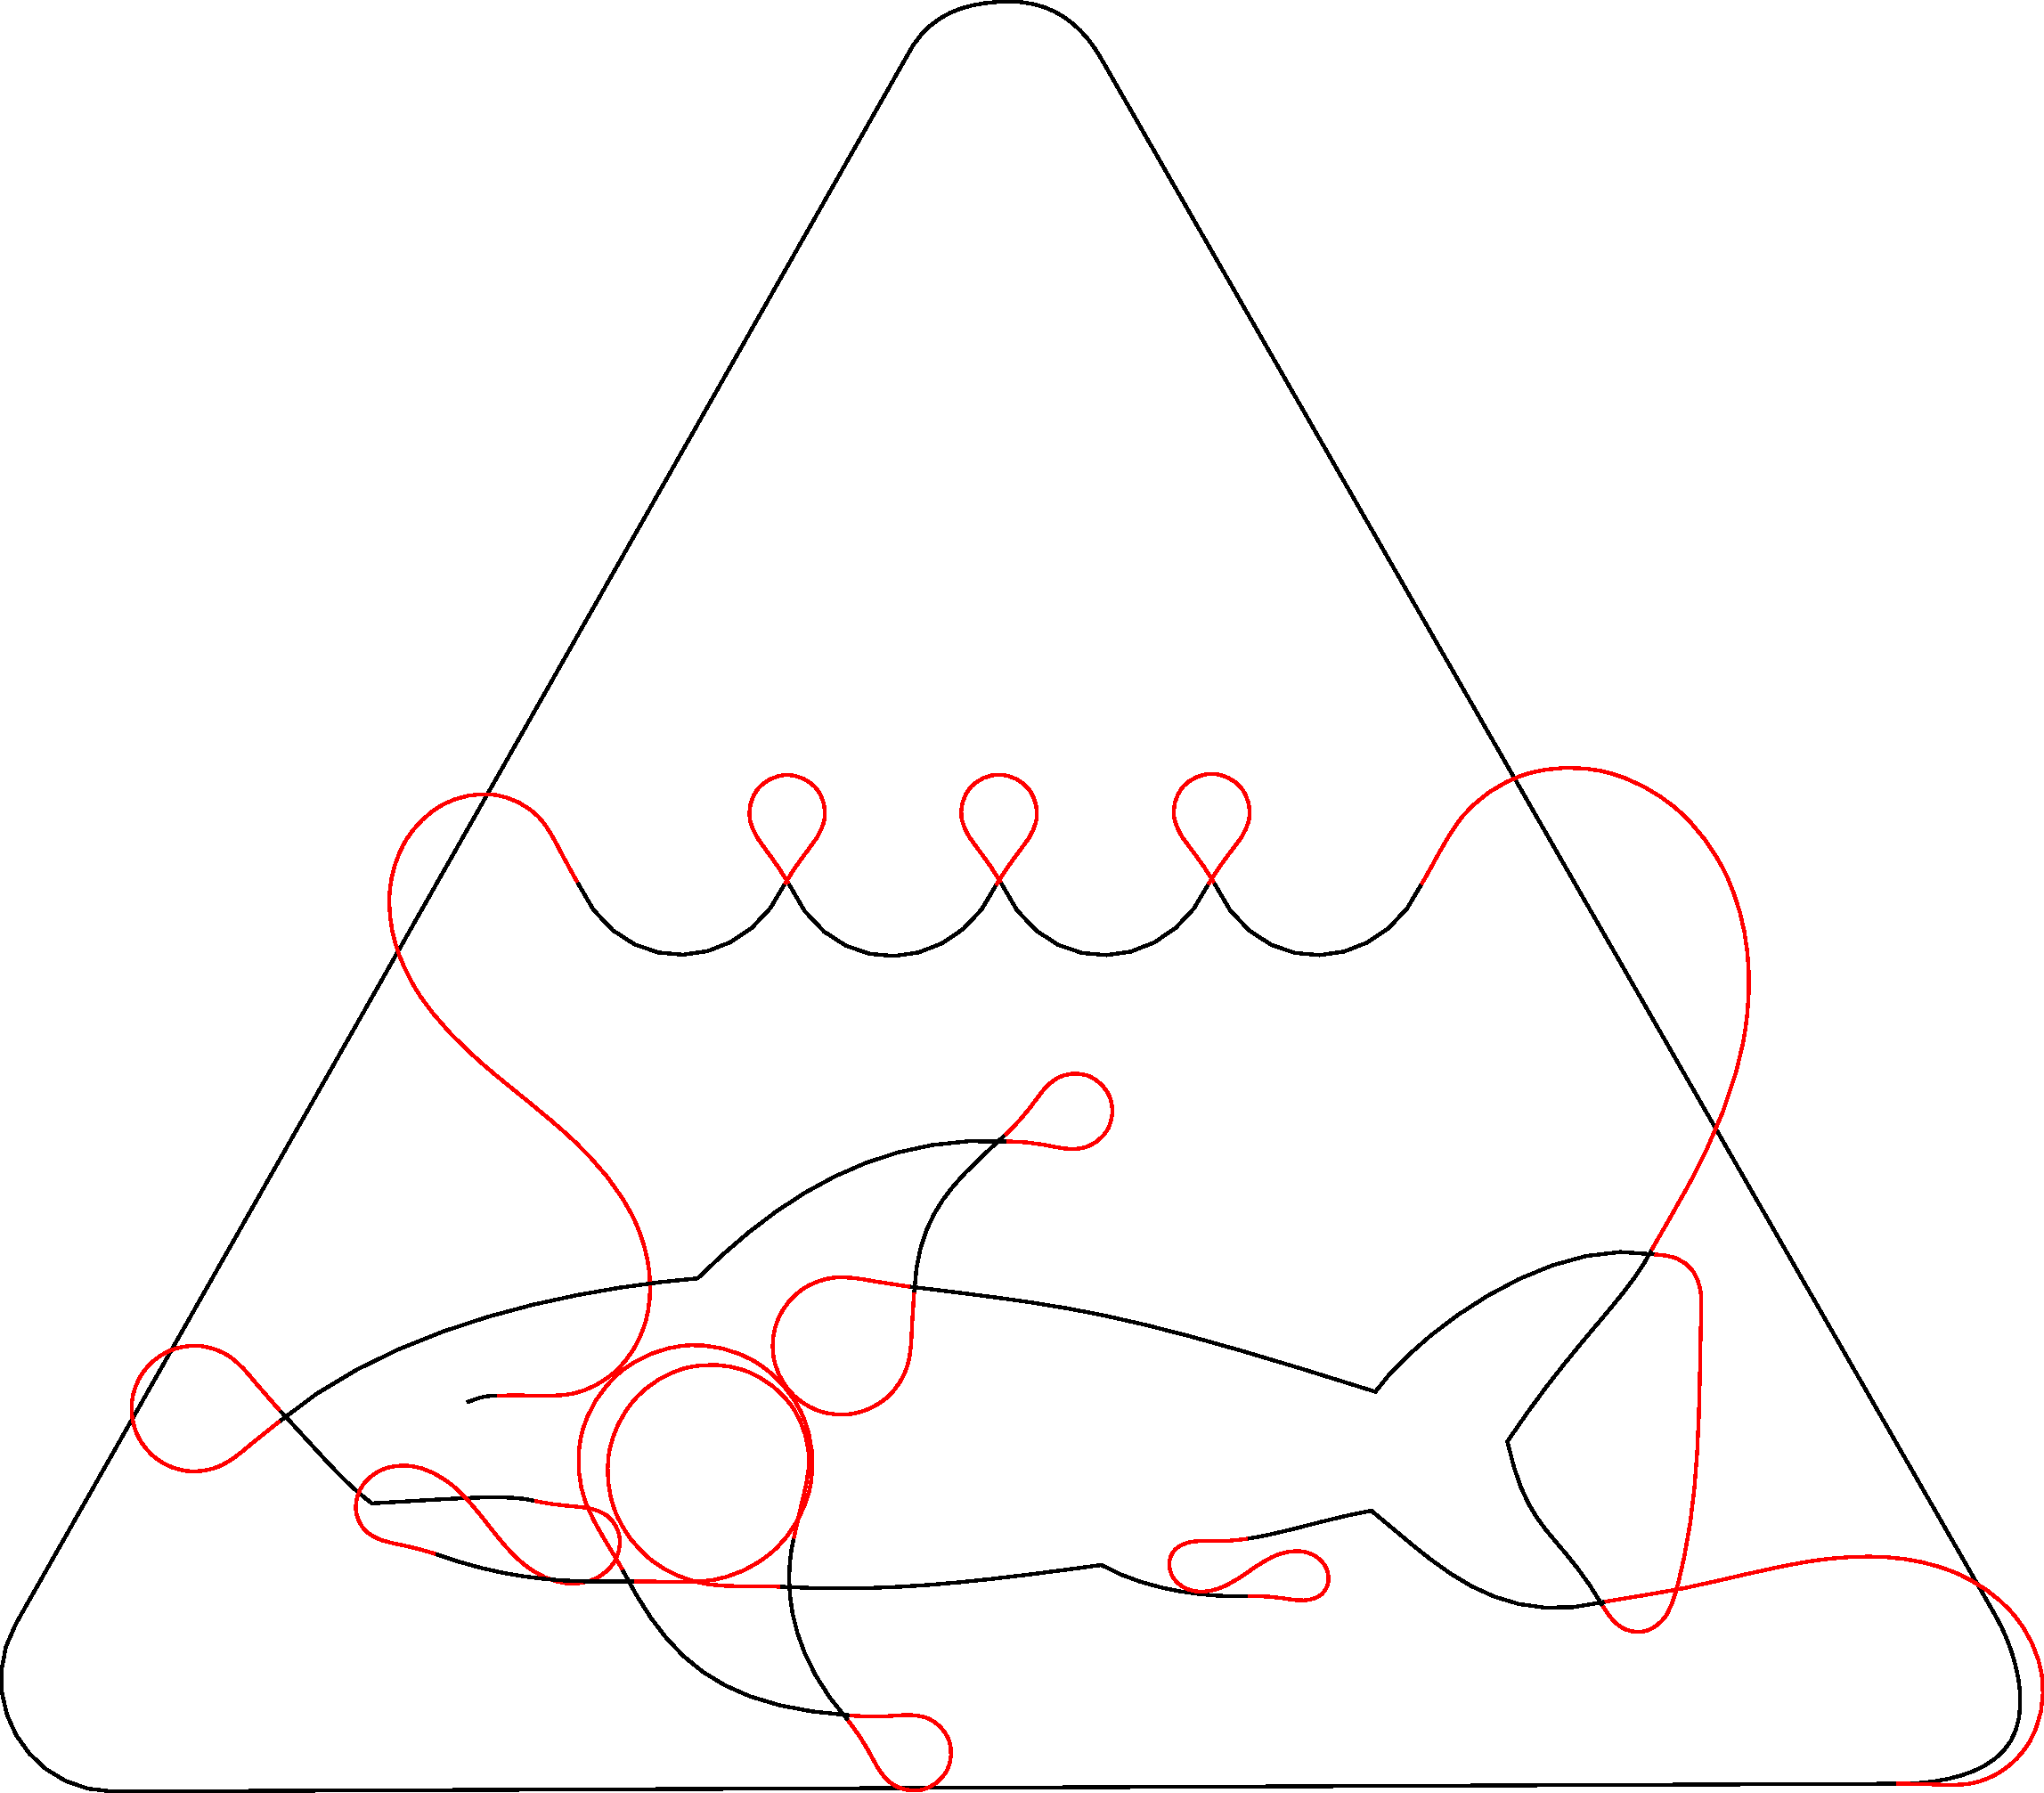
\includegraphics[width=\textwidth]{images/results/shark/shark_prevent_outer.pdf}
	\caption{Generated by the path generator. This time, the enclosing polygon is entered last (by modifying the distance matrix as described in \autoref{sec:cont}}.
\end{subfigure}

\caption{Comparison of manual and automatically generated \textit{Danger, Shark} trajectory}
\end{figure}

\clearpage
\subsection{Fonts}

\textit{Inkscape} has an extension called Hershey Text\footnote{\url{http://www.evilmadscientist.com/2011/hershey-text-an-inkscape-extension-for-engraving-fonts/}}, which offers a variety of engraving fonts that have been designed by Hershey in 1967 \cite{hershey1967calligraphy}. While designed for the purpose of being engraved to metal or stone, they are equally well suited to be drawn on sand. There are variants of each font, from single line to three lines per letter. As of now, only the single line variant has been tested with the path generator. For the single line variant two different styles are available: script and sans-serif.

\begin{figure}[h]
\centering
\begin{subfigure}[t]{0.95\textwidth}
\centering
	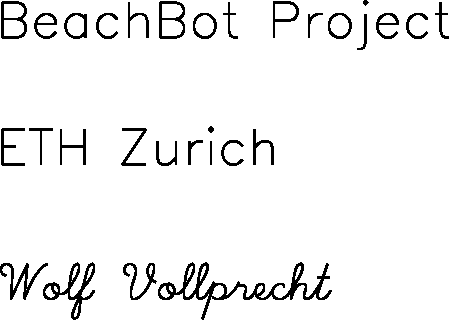
\includegraphics[width=\textwidth]{images/results/hershey/hershey_text.pdf}
	\caption{Example text set with sans-serif and script font.}
\end{subfigure}
\par \bigskip
\begin{subfigure}[t]{0.95\textwidth}
\centering
	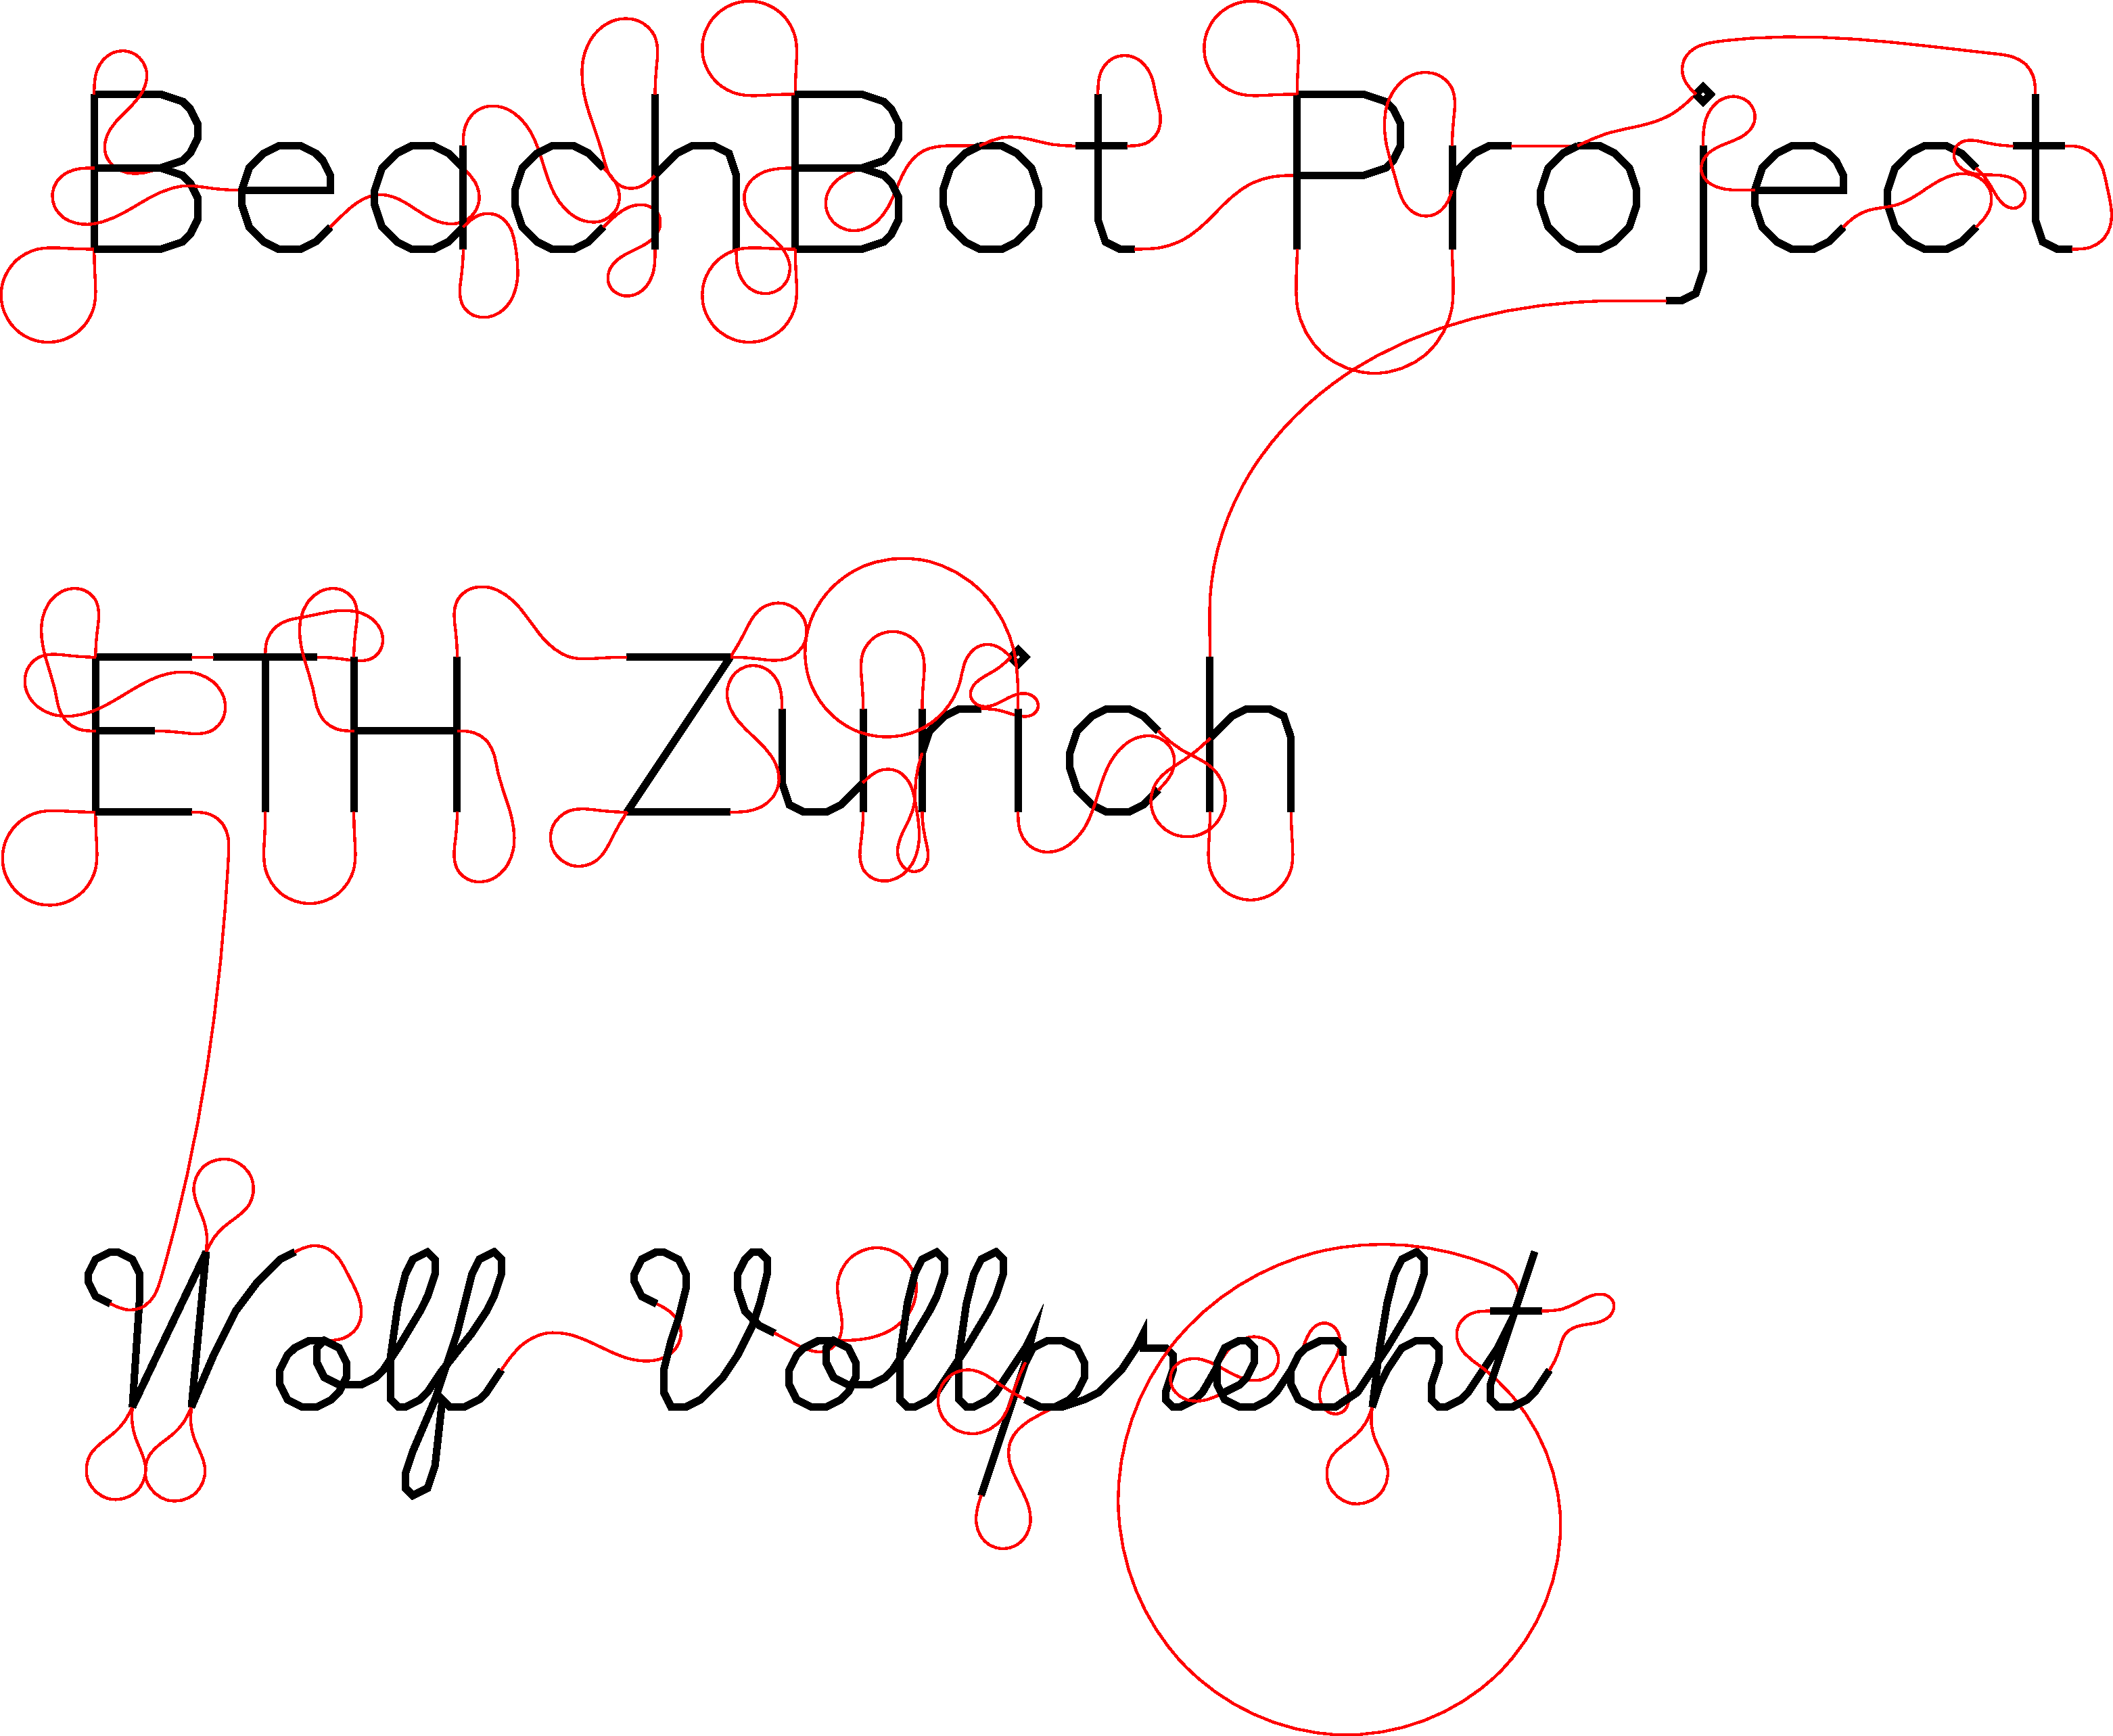
\includegraphics[width=\textwidth]{images/results/hershey/hershey_connected.pdf}
	\caption{The connected drawing.}
\end{subfigure}

\end{figure}

\clearpage

\section{Drawings with Filled Areas}
\subsection{ASL Logo}

\begin{figure}[h]
\centering
\begin{subfigure}[t]{0.95\textwidth}
\centering
	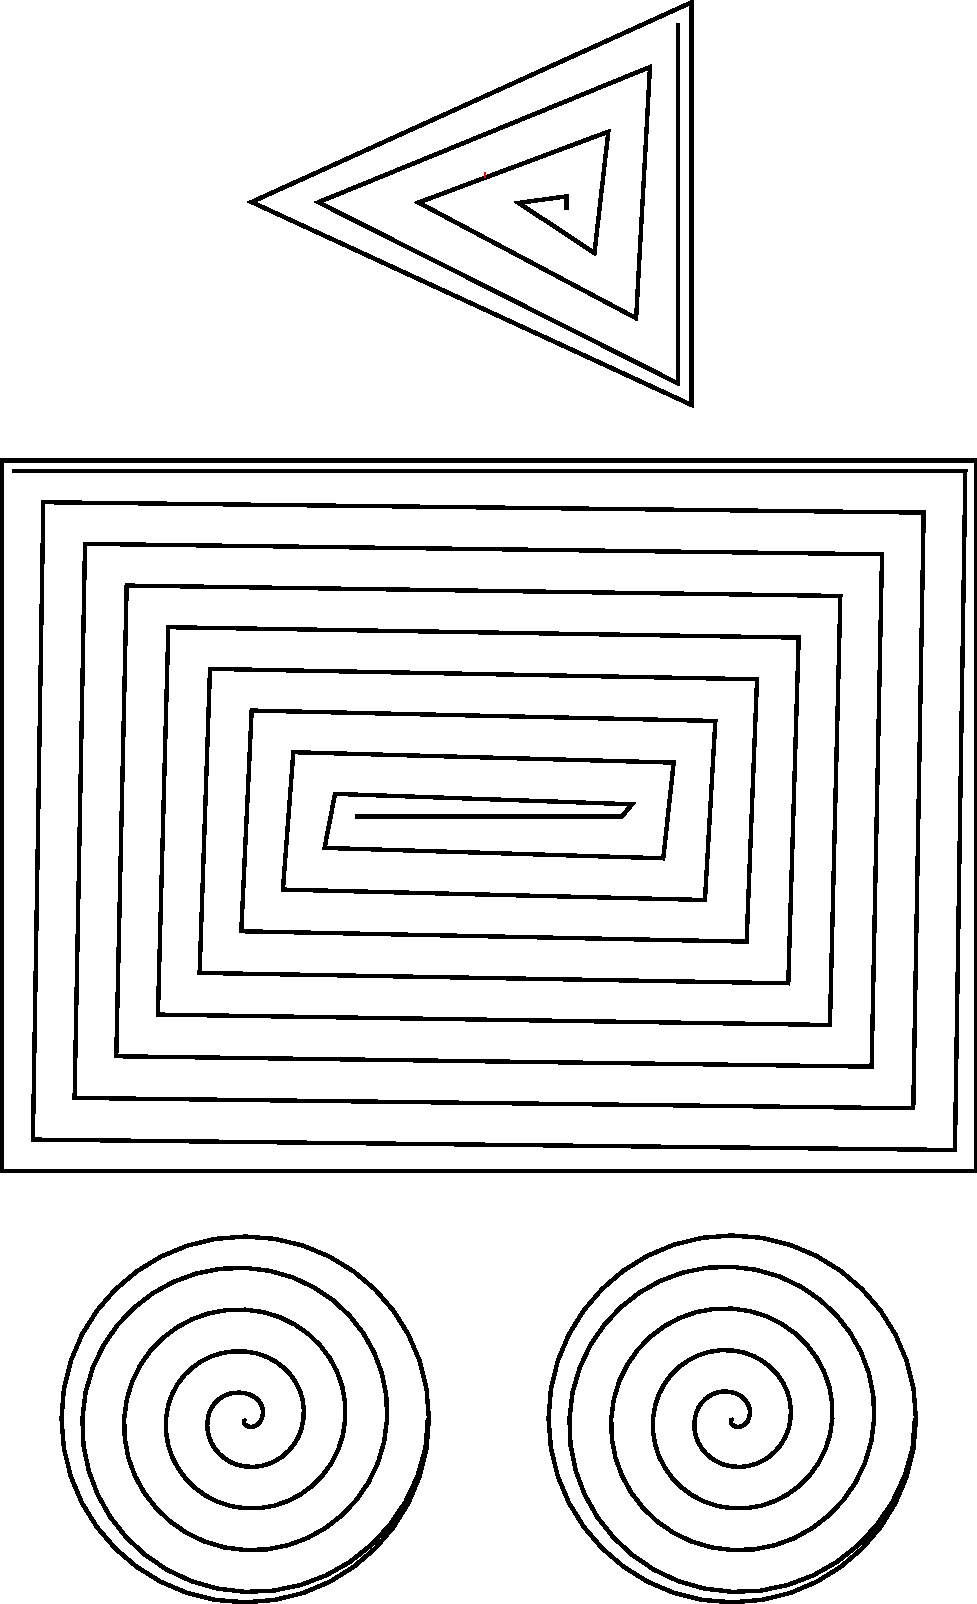
\includegraphics[height=9cm]{images/results/asl/asl_logo_spiral.pdf}
	\caption{ASL Logo areas filled by generated spirals.}
\end{subfigure}\\
\begin{subfigure}[t]{0.95\textwidth}
	
\includegraphics[width=\textwidth]{images/results/asl/asl_font.pdf}
	\caption{ASL written in a highly concave font.}
\end{subfigure}
\caption{Comparison of manual and automatically generated \textit{Danger, Shark} trajectory}
\end{figure}

%\subsection{A \textit{Maleficient} Character}

%\begin{figure}[h]
%\centering
%\begin{subfigure}[t]{0.95\textwidth}
%\centering
%	
\includegraphics[width=\textwidth]{images/results/mal/maleficient_source.pdf}
%	\caption{Source bitmap image and manually traced vector graphics (right). All rights to the \textit{Maleficent} character and the image reserved by \textcopyright Disney.}
%\end{subfigure}\\
%\begin{subfigure}[t]{0.95\textwidth}
%\centering
%	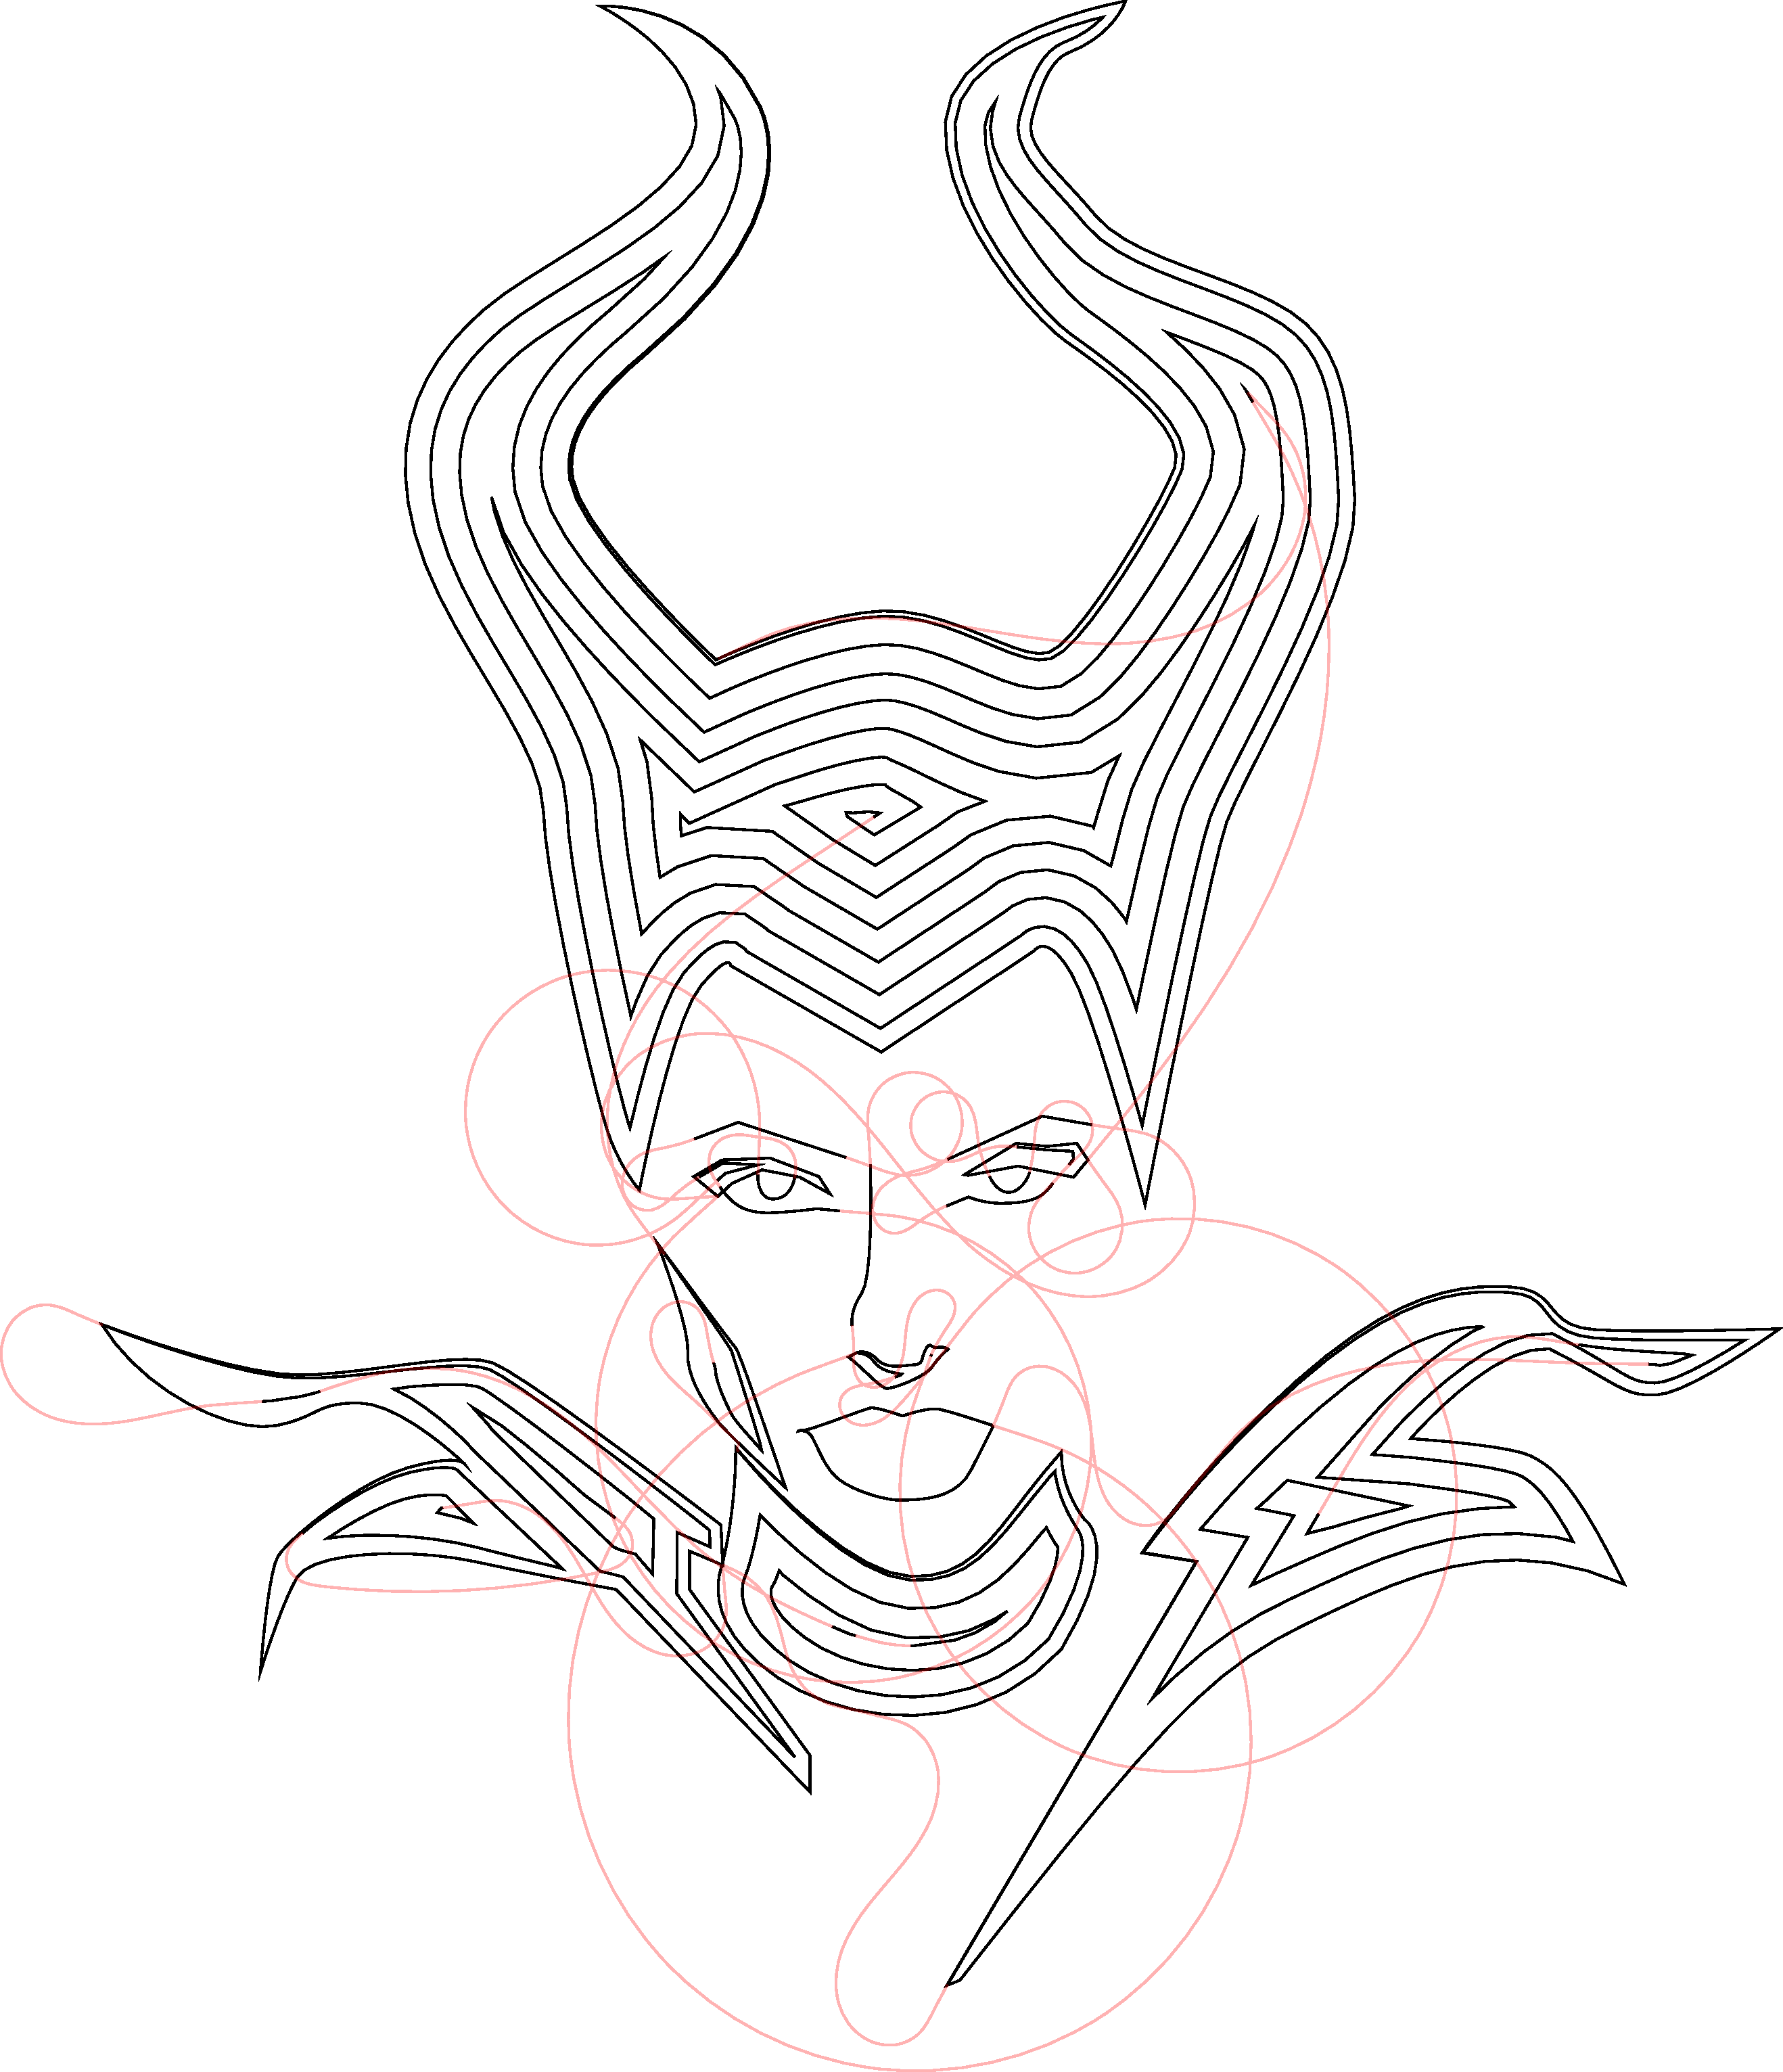
\includegraphics[width=\textwidth]{images/results/mal/maleficient.pdf}
%	\caption{Generated trajectory. Note that the mouth is not filled due to a small error in the traced vector graphics.}
%\end{subfigure}
%\caption{A drawing depicting the main character of the upcoming \textit{Maleficent} (\textcopyright Disney) movie. First, a vector graphic has to be manually created, using a bitmap as reference. Based on the vector graphic, a trajectory can be generated.}
%\end{figure}